%----------------------------------------------------------------------------------------
%	PACKAGES AND OTHER DOCUMENT CONFIGURATIONS
%----------------------------------------------------------------------------------------
\documentclass[fleqn,9 pt]{SelfArx} % Document font size and equations flushed left

% Decrease margins
%\addtolength{\oddsidemargin}{-0.3 in}
%\addtolength{\evensidemargin}{0 in}
%\addtolength{\textwidth}{0.8 in}
%\addtolength{\topmargin}{-0.5 in}
%\addtolength{\textheight}{1 in}

\usepackage[english]{babel} % Specify a different language here - english by default
\usepackage{lipsum} % Required to insert dummy text. To be removed otherwise
\usepackage{listings}
\usepackage{lipsum}  
\usepackage{caption}

%----------------------------------------------------------------------------------------
%	COLUMNS
%----------------------------------------------------------------------------------------
\setlength{\columnsep}{0.55cm} % Distance between the two columns of text
\setlength{\fboxrule}{0.75pt} % Width of the border around the abstract
%----------------------------------------------------------------------------------------
%	COLORS
%----------------------------------------------------------------------------------------
\definecolor{color1}{RGB}{0,0,90} % Color of the article title and sections
\definecolor{color2}{RGB}{0,20,20} % Color of the boxes behind the abstract and headings

%----------------------------------------------------------------------------------------
%	HYPERLINKS
%----------------------------------------------------------------------------------------
\usepackage{hyperref} % Required for hyperlinks
\hypersetup{hidelinks,colorlinks,breaklinks=true,urlcolor=color2,citecolor=color1,linkcolor=color1,bookmarksopen=false,pdftitle={Title},pdfauthor={Author}}

%----------------------------------------------------------------------------------------
%	ARTICLE INFORMATION
%----------------------------------------------------------------------------------------
\JournalInfo{Mini-project 1 - CS-433 - Pattern Classification and Machine Learning} % Journal information
\Archive{\today} % Additional notes (e.g. copyright, DOI, review/research article)

%%%%% dumb test
\usepackage[english]{babel}
\usepackage{blindtext}

\PaperTitle{The Higgs boson machine learning challenge} % Article title

\Authors{Bruno Magalhaes\textsuperscript{1}, Riccardo Silini{2}} % Authors
\affiliation{\textbf{Email (SCIPER):} \hspace{0.2cm} \textsuperscript{1} bruno.magalhaes@epfl.ch (212079) \hspace{0.2cm} \textsuperscript{2} riccardo.silini@epfl.ch (214398) \hspace{0.2cm}}

\Keywords{}
%Keyword1 --- Keyword2 --- Keyword3

\newcommand{\keywordname}{Keywords} % Defines the keywords heading name

%to allow overlapping
\usepackage[percent]{overpic}
\usepackage[]{algorithmic,algorithm2e}

%to allow \figures right below text 
\usepackage{float}

%---------- ABSTRACT

\Abstract{ \small
bla bla bla
}

\begin{document}
\begin{sloppypar} %allows line breaks in \texttt{---} section

\flushbottom % Makes all text pages the same height
\maketitle % Print the title and abstract box
%\tableofcontents % Print the contents section
%\thispagestyle{empty} % Removes page numbering from the first page

\section{Introduction}


\section{Data Augmentation}
\label{sec-pre-proc}

\paragraph{1. Rotation of input images with non-orthogonal roads} We increased the number of input images from $100$ to $148$ by rotating $90 \deg$, $180 \deg$ and $270 \deg$ the (16) training images that are not composed only of non-horizontal and non-vertical roads. This feature is activated by the flag \texttt{DATA\_AUGMENTATION}.

\paragraph{2. Patches from concatenation points} We increase by almost two-fold the number of patches per training image by performing extraction of all patches of size \texttt{IMG\_PATCH\_SIZE} that are placed at every \texttt{IMG\_PATCH\_SIZE/2} interval. This feature is activated by the flag \texttt{ADD\_INTERCALATED\_PATCHES}. In practice, it extracts patches with the corners at the mid-point positions of previously extracted patches, as displayed below:

\begin{figure}[H]
\centering
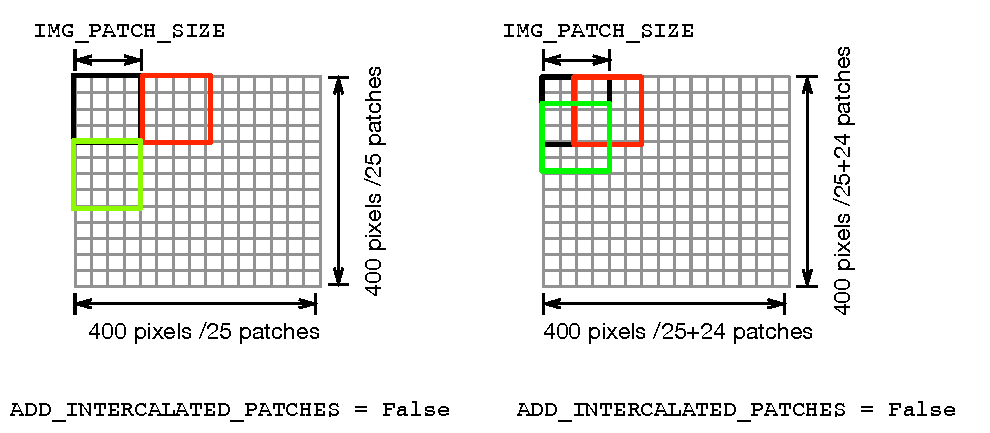
\includegraphics[width=0.47\textwidth]{figures/ADD_INTERCALATED_PATCHES.pdf}
\caption{\small The collection of patches by stepping \texttt{IMG\_PATCH\_SIZE} (default, left) compared with \texttt{IMG\_PATCH\_SIZE/2} (\texttt{ADD\_INTERCALATED\_PATCHES} activated, right). When traversing image, next collected patch on the horizontal (vertical) direction is displayed as red (green).}
\end{figure}

\section{Features}

\paragraph{Two-step classification} 

To reduce noise and allows classification at a finer scale, we added a second neural network to the processing. The initial one will be trained with pairs of [images,groundtruth] and outputs the segmented classification. The second network is trained with pairs [classification,groundtruth] and received the first network's classification as input, outputting the final classification. The second step of this operation is presented as \texttt{Phase 2} in the source code. An example of an application of the two-step classification is displayed in the following picture.

\begin{figure}[H]
\centering
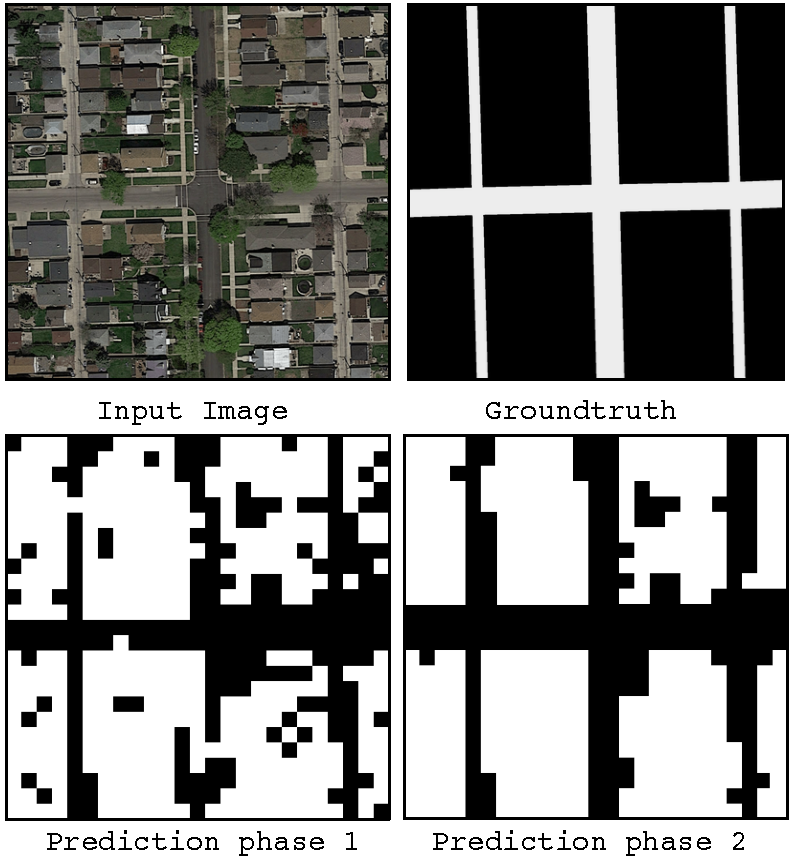
\includegraphics[width=0.3\textwidth]{figures/two_phases_conv2d.pdf}
\caption{\small An example of the application of the two-phase propagation process: for a given input (top-left), the predicted segmentation at output of the neural network (bottom-left) is then re-input to a second neural network trained from groundtruth images (top-right), outputting the final classification (bottom-right).}
\end{figure}

\paragraph{Analysis of neighborhood information} This functionality can be activated wit the flag \texttt{NEIGHBORHOOD\_ANALYSIS} set to \texttt{True} and definining the \texttt{NEIGHBOR\_PIXELS} to the margin of neighborhood pixels to be added and analysed from each patch.

\begin{figure}[H]
\centering
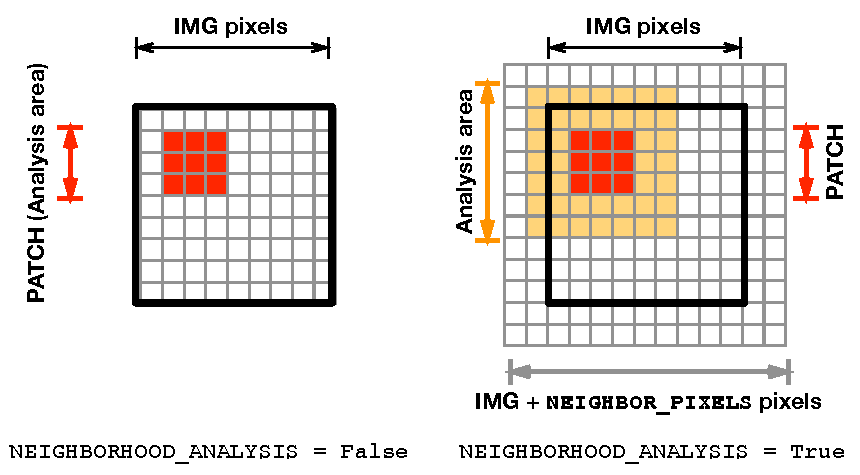
\includegraphics[width=0.47\textwidth]{figures/NEIGHBORHOOD_ANALYSIS.pdf}
\caption{\small Example of the neighborhood analysis feature. Standard classification (left) inputs patches of images and classifies the same area. With neighborhood analysis (right), we input the patch of size \texttt{IMG\_PATCH\_SIZE} and all surrounding \texttt{NEIGHBOR\_PIXELS} pixels (orange), with the learning based on the labels of the patch only (red).}
\end{figure}

\paragraph{Randomized input sequence}

The order in which we present the observations (input vectors) comprising the training set to the network affects the final computation of weights. We implemented a randomized arrangement of the observations according to the response variable that has been shows to be present a better tuned network when compared with ordered arrangements (the standard implementation). Our input is then a randomized set of classification with balanced number of inputs for each label. This feature is enabled by defining \texttt{RANDOMIZE\_INPUT\_PATCHES = True}.

\paragraph{Dropout}

Dropout is a regularization technique for reducing the overfitting of neural networks. It performs model averaging of neural networks efficiently and prevents complex co-adaptations on training data (Srivastava et at. 2014 \cite{srivastava2014dropout}). We enabled dropout in our models by specifying the percentage of dropout on the variable \texttt{DROPOUT\_RATE} as exemplified in the next figure:

\begin{figure}[H]
\centering
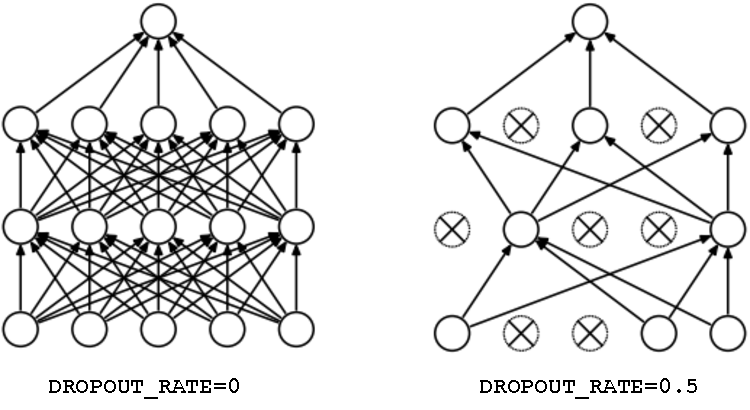
\includegraphics[width=0.44\textwidth]{figures/DROPOUT_RATE.pdf}
\caption{\small Example of the dropout feature. Standard weights tunning (left) methods apply an update of all weights. Dropout-based networks (right) discards the updates of certain weights with the rationale of reducing overfitting. In the example, a dropout rate of \texttt{0.5} disables half of the nodes on the network.}
\end{figure}

\paragraph{Multi-Layer convolutional network}

We allow the sub-network of convolution layers to increase or decrease, according to the user-defined parameters \texttt{CONV\_LAYERS}. This allowed us to play with the quality of model fitting for different set set of parameters. In practice, our network is an array of convolution and pooling layers, where the output of one layer is the input of the following one. The parameters of every layer is fully customisable by the user from the following variables:
\begin{itemize}
\item \texttt{CONV\_LAYERS}: number of convolutional layers, and size of the following parameter arrays;
\item \texttt{CONV\_FILTER\_SIZES = [5,5,5,5]} : For each layer, the count of horizontal and vertical pixels of filter;
\item \texttt{CONV\_FILTER\_DEPTHS = [32, 64, 128, 256]}: depth of the weights for the aforementioned layers;
\item \texttt{POOL\_FILTER\_STRIDES = [2, 2, 2, 2]}: horizontal and vertical stride for the max-pooling on each layer;
\item \texttt{FC1\_WEIGHTS\_DEPTH = 512}: depth of the first fully connected layer, connected to conv. layer of id \texttt{CONV\_LAYERS-1}. The second layer performs binary probability classification therefore has depth \texttt{NUM\_LABELS} (road; non-road);
\end{itemize}
  This allowed us to play with the quality of fitting based on user-provided filter sizes, depths and strides -- as detailed in the following paragraph.

\paragraph{Final Network Architecture}

In brief, our network is composed by a set of convolution layers (for extracting of convoluted features) and pooling layers (for the extraction of most meaningful weights from convolutional layer outputs), followed by two layers of fully connected layers (the universal function approximators). The input is a set of images to which patches are extracted. Those patches are then input individually or in batches to the network. The output contains the probability of the road or non-road classification. A sample of a possible network architecture with 2 convoluted layers and default parameters is displayed in figure \ref{fig-conv-2d-architecture}.

\begin{figure*}
\centering
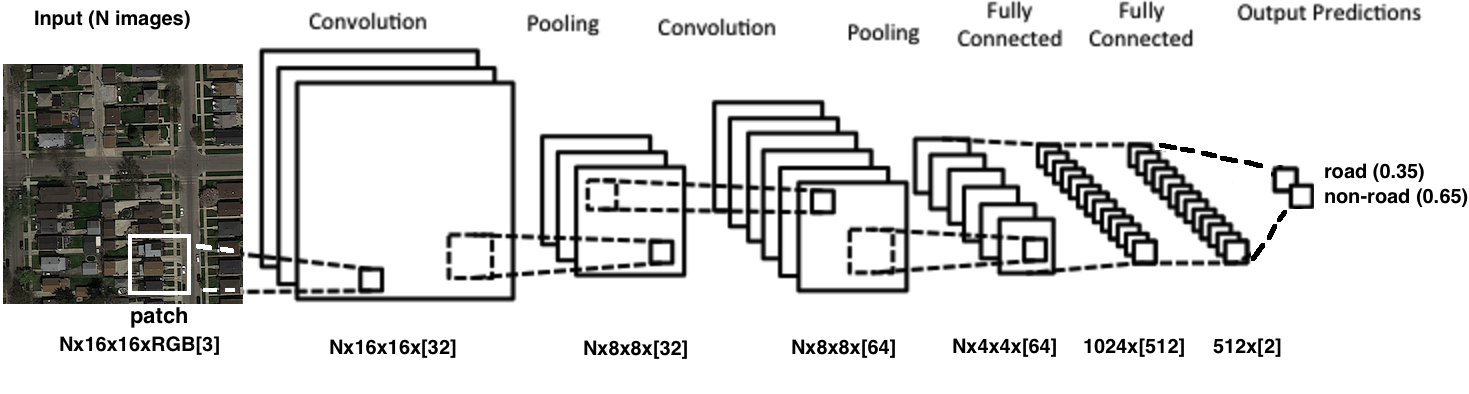
\includegraphics[width=0.9\textwidth]{figures/conv_2d_network.png}
\caption{\small A general overview of the deep network architecture, with default parameters. Dimensionalities, padding types, depths and number of convolution+pooling layers are user-customisable.}
\label{fig-conv-2d-architecture}
\end{figure*}

\section{Performance Analysis and Results}

Riccardo bla bla bla

\section{Final Remarks and Conclusion}
\label{sec-Conclusion}

bla bla bla 


%references
\bibliographystyle{unsrt}
\bibliography{report}

\end{sloppypar}
\end{document}